\begin{cabstractextra}
    本文提出基于实例分割的多人姿态估计网络结构,能够在单张图像上准确提取多人人体姿态信息,从而实现序列图像多人姿态的检测与跟踪。所提出结构通过双任务的深度融合,能够借助实例分割线索区分不同人体区域,更好地解决多人姿态估计中的遮挡问题;同时,借助姿态检测结果反向优化实例分割。为了有效区分不同人体区域,所提出网络结构在其姿态估计分支中引入注意力机制。鉴于现有可用的实例分割真值缺失人体被遮挡部分的数据,难以用于人体区域注意力的生成,本文引入弱监督学习策略,使用来自关键点与实例分割的两个损失函数间接约束注意力产生过程,以鼓励被遮挡区域的生成。
\end{cabstractextra}
\begin{eabstractextra}
    In this work, we propose a novel deep learning architecture for multi-person pose estimation. It can locate multi-persons in single images, thereby achieving multi-person pose detection and tracking in image sequences. It integrates information from instance segmentation, by generating spatial attention to merge features from the two tasks. The proposed architecture effectively improves both pose estimation and instance segmentation. In order to distinguish difference instances, we utilize attention mechanism in the proposed network. Since it is incomplete in occluded body parts, the ground truth of instance segmentation cannot be used to supervise the training of spatial attention. We train the attention module with weakly supervised learning techniques. This stimulates the proposed network to successfully extract poses in occluded body parts.
\end{eabstractextra}
\begin{outstandingabstract}
    \section{绪论}
	人体姿态检测与跟踪旨在从传感器数据中捕捉多人姿态信息,在各领域具有广阔的应用前景,其中部分技术在特定场景中已得以应用。与基于组合传感器的姿态采集与追踪设备相比,基于单目相机的多人姿态估计方法不受限于室内场景,应用更加广泛,因此拥有更高的研究价值与应用前景。然而,基于单目相机的多人姿态提取面临诸多技术难点,其中最难以解决的是多人场景中的互遮挡问题。现有多人姿态估计方法在不同个体躯干相互遮挡的情况下,难以根据可视部分推断不可见部分的信息,从而确定被遮挡部位的姿态。例如,当图像中的特定人肩部被遮挡时,现有算法难以给出其准确的肩部位置。鉴于上述事实,本文在研究现有姿态估计方法的基础上,提出基于实例分割的多人姿态估计方法,从而更好地解决多人姿态估计过程中的互遮挡问题,实现准确的多人姿态检测与跟踪。
	
	
    \section{基于实例分割的多人姿态估计方法}
	本方法使用基于残差网络\cite{He2015Deep}与特征金字塔网络\cite{Lin2016Feature}结构的网络框架作为特征提取的骨架,为模型提供各个尺度的特征图。在特征提取部分之后,网络可以被分为目标检测与姿态估计和融合回归两个网络。在检测部分中,网络预测目标的边界、粗略的关键点预测和实例分割结果。在融合优化网络中,算法接受从检测部分产生的结果并将两任务中生成的特征交汇并一同回归。
	
	本文采取了多阶段堆叠和中继监督策略来共同优化关键点与实例分割的结果\cite{wei2016convolutional}。同时,为了有效地融合实例分割与姿态估计,本文引入注意力机制,使其根据由实例分割生成的注意力关注特定人体实例的区域,从而达到解决多人场景下遮挡问题的目标。考虑到姿态估计的信息对实例分割有促进作用,本文设计联合优化的网络结构让模型在每个阶段都能同时预测分割结果和姿态估计结果,并送入下一阶段继续优化。
 
 	\subsection{检测模块}
 	本文网络设计中的检测模块由特征提取网络与检测回归网络两部分组成。在特征提取网络中本文使用了残差网络作为特征提取的基础结构。同时,本文为了更好地融合来自不同尺度的特征,还使用了特征金字塔\cite{Lin2016Feature}来自底向上地融合不同尺寸的特征。检测回归网络是由两个并行的分支组成的。实例分割分支与姿态估计分支分别使用裁剪好的特征得到粗略的实例分割结果与姿态估计结果。
 	
 	\subsection{融合优化网络}
 	本文设计了多个具有相同结构的优化模块同时优化实例分割与姿态估计。本文提出的优化模块通过引入考虑遮挡区域的软注意力,强化对应区域的特征响应,从而改善网络在遮挡情况下对人体姿态信息的提取能力。同时软注意力用来增强实例分割的特征表达,将分割信息在模块间传递并优化。
 	\subsubsection{优化模块结构设计}
 	优化模块结构设计如图\ref{fig:RefineNet}所示。优化模块的设计有两个目标,一个是将多任务的每个分支的信息从当前阶段传递到下一个阶段;另一个目标是网络应该有较好的融合方法让两个任务的特征。对于第一个目标,网络结构在每个分支都设计了传递的结构,以增强每个阶段在现有结果上优化的能力;其次,本文对于两个任务特征融合也对应设计了融合方法以达到交叉优化的目标。所以本文提出了涉及了多个拥有相同结构的优化模块多阶段地融合关键点信息与分割信息以增强姿态估计与实例分割的最终结果。
 	\begin{figure*}[h]	
 		\centering
 		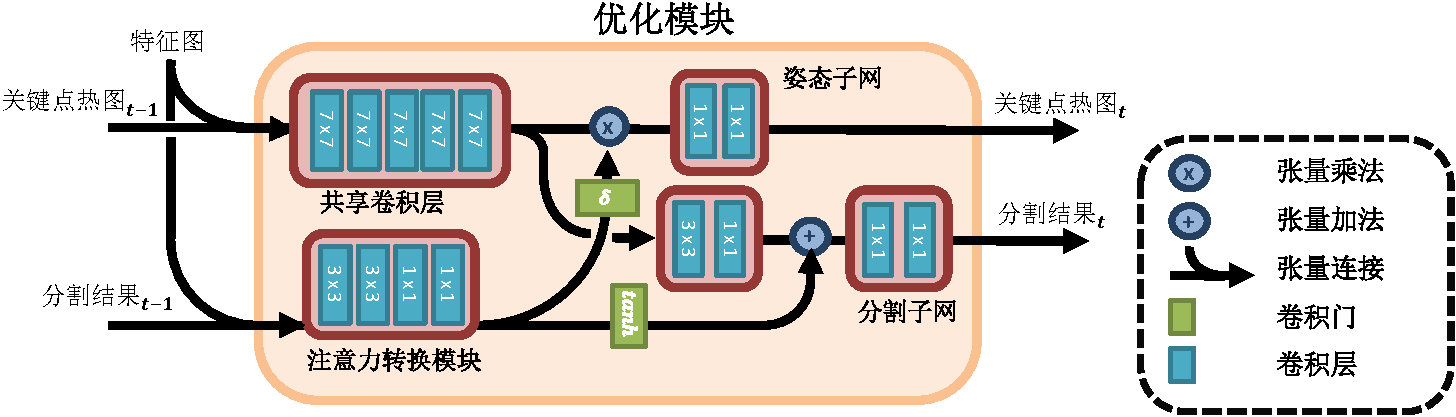
\includegraphics[width=\textwidth]{RefineNet.pdf}
 		\caption{融合优化网络具体设计}
 		\label{fig:RefineNet}
 	\end{figure*}
 
 	\subsubsection{弱监督与注意力机制}
 	本文使用了弱监督方法约束空间注意力的生成\cite{10.1093/nsr/nwx106}。来自实例分割的标注真值未能将被遮挡的人体区域考虑在内,因此空间注意力为了学习遮挡区域的生成不能在实例分割监督信息的直接约束下训练得到。然而关键点任务的真值标注给出了部分被遮挡人体区域的关键点信息。本文以空间注意力为桥梁网络结构设计,将两任务分支交叉连接,在联合损失函数的共同作用下,间接约束网络生成考虑遮挡的空间注意力。在互补的监督信息以及弱监督的约束下,空间注意力能够很好地补全被遮挡的人体区域,从而在空间上选择并强化两任务中对应位置的特征。
 	
 	\subsection{网络训练}
 	本文监督网络的损失函数可以被分为三部分:边界框损失函数、关键点分支损失函数与实例分割损失函数\footnotemark[1]。为了平衡每个分支的收敛速率,本文设计了$\beta$和$\alpha$分别控制目标检测与实例分割的损失函数权重\footnotemark[1]。由于本文提出的优化模块结构涉及到两支输出相互交叉与传递,因此给出了损失函数中不同项对于梯度的影响,从而证明了网络能够在添加结构的条件下保证两支网络的正常收敛\footnotemark[1],也解释了弱监督信息能使用两任务联合损失函数监督注意力的生成。
 	
 	\footnotetext[1]{具体描述请参考论文}
 	
	    
    \section{实验验证与分析}
	本文在COCO2017数据集上对比了现有方法与本文方法的性能指标,并通过设计多个对比消融实验分别证明了本文中提出的优化模块的有效性。通过大量定量与定性实验展示网络模型同时给出分割结果和姿态估计结果的性能,并证明本文提出弱监督下空间注意力的有效性。
    
    \subsection{视觉效果与分析}
    
    \begin{figure}[H]
    	\centering
    	\begin{minipage}{\linewidth}
    		\centering
    		\begin{subfigure}[b]{0.45\linewidth}
    			\centering
    			\begin{minipage}{\linewidth}
    				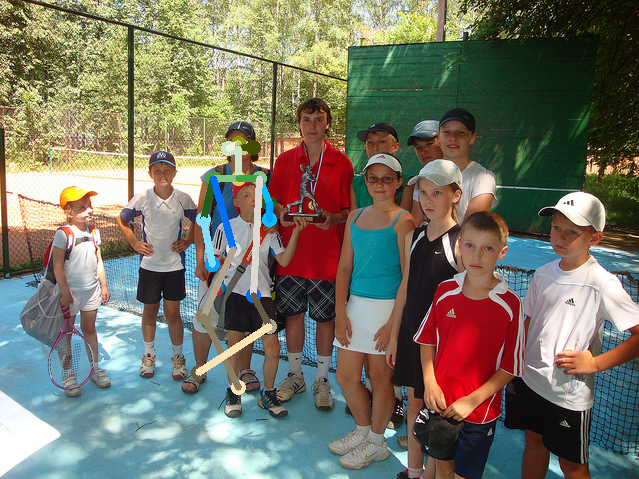
\includegraphics[width=0.48\linewidth]{1000_insid9_stage3_keypoint_baseline.png}
    				\adjustbox{width=0.48\linewidth, trim={.1\width} {.1\height} {.25\width} {.25\height},clip}
    				{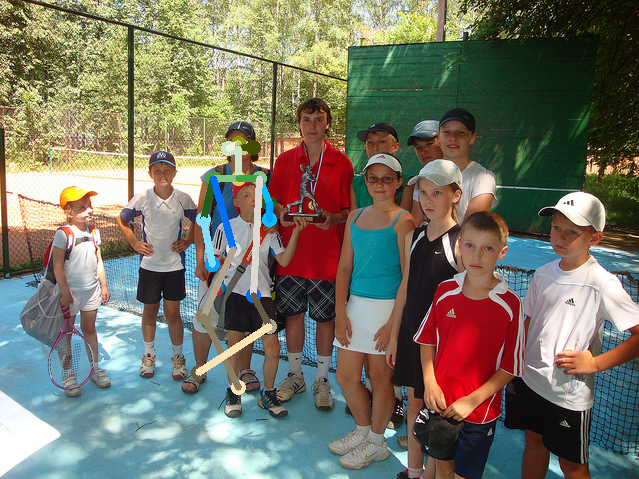
\includegraphics[width=\linewidth]{1000_insid9_stage3_keypoint_baseline.png}}
    			\end{minipage}
    		\end{subfigure}
    		\begin{subfigure}[b]{0.45\linewidth}
    			\centering
    			\begin{minipage}{\linewidth}
    				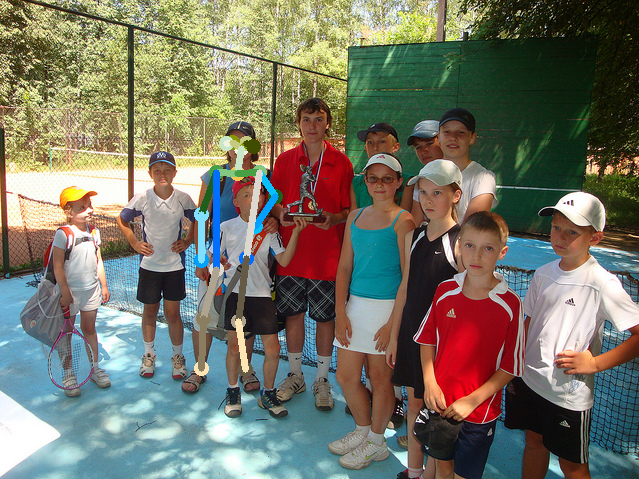
\includegraphics[width=0.48\linewidth]{1000_insid9_stage5_keypoint.png}
    				\adjustbox{width=0.48\linewidth, trim={.1\width} {.1\height} {.25\width} {.25\height},clip}
    				{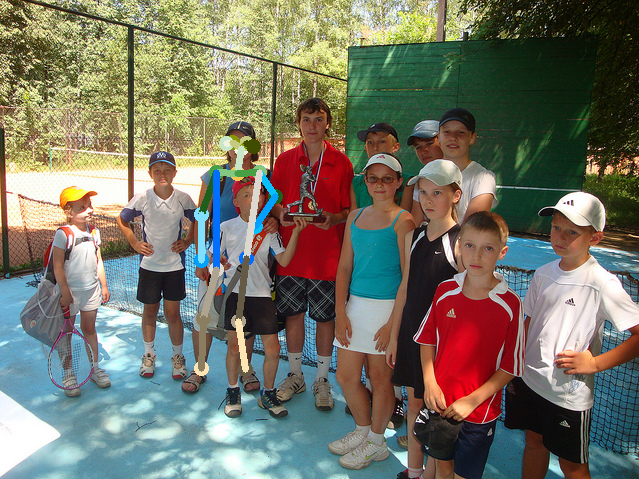
\includegraphics[width=\linewidth]{1000_insid9_stage5_keypoint.png}}
    			\end{minipage}
    		\end{subfigure}
    		
    		\vskip5pt
    		\begin{subfigure}[b]{0.45\linewidth}
    			\centering
    			\begin{minipage}{\linewidth}
    				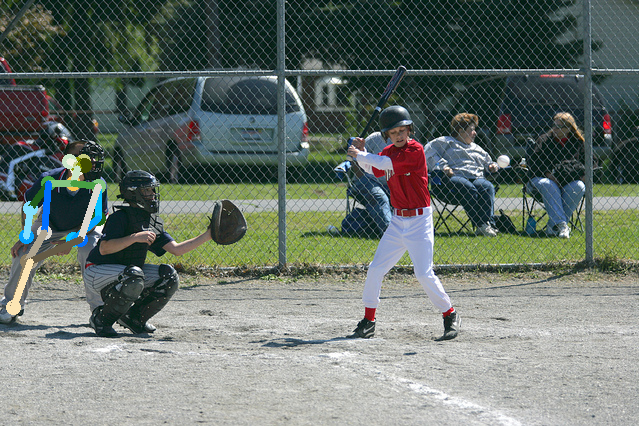
\includegraphics[width=0.48\linewidth]{54593_insid3_stage3_keypoint_baseline.png}
    				\adjustbox{width=0.48\linewidth, trim=0 {.2\height} {.4\width} {.2\height},clip}
    				{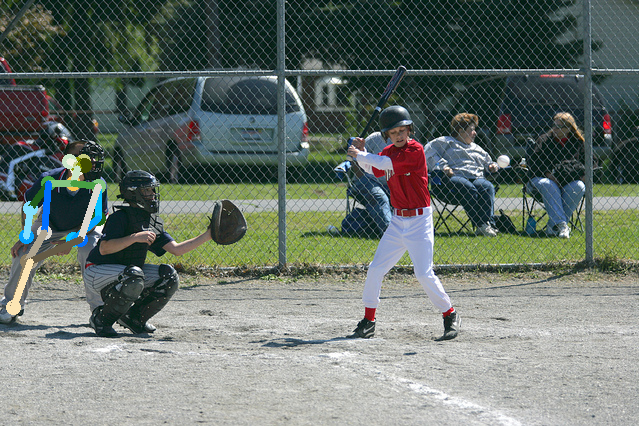
\includegraphics[width=\linewidth]{54593_insid3_stage3_keypoint_baseline.png}}
    			\end{minipage}
    			\caption{基准方法\cite{wei2016convolutional}}
    		\end{subfigure}
    		\begin{subfigure}[b]{0.45\linewidth}
    			\centering
    			\begin{minipage}{\linewidth}
    				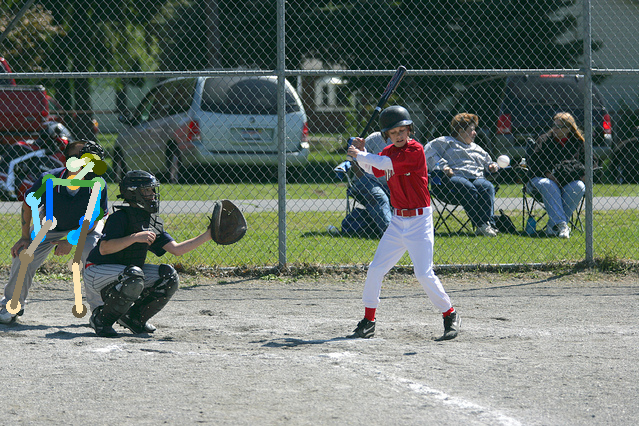
\includegraphics[width=0.48\linewidth]{54593_insid3_stage5_keypoint.png}
    				\adjustbox{width=0.48\linewidth, trim=0 {.2\height} {.4\width} {.2\height},clip}
    				{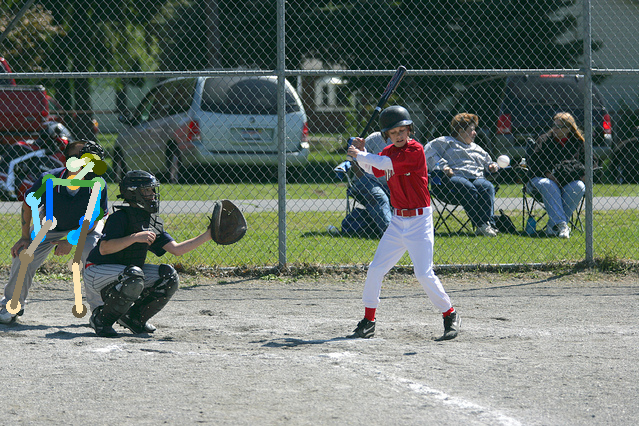
\includegraphics[width=\linewidth]{54593_insid3_stage5_keypoint.png}}
    			\end{minipage}
    			\caption{本文方法}
    		\end{subfigure}
    	\end{minipage}
    	\caption{本文方法与基准方法关键点任务对比视觉效果图}
    	\label{fig:comparison_keypoint}
    \end{figure}
	如图\ref{fig:comparison_keypoint}所示,本文方法可以比基准方法更好地关注单个实例。通过自生成空间注意力约束,本文方法能够给出更加规整的关键点预测结果,并将结果限制于有限的特定人体区域内。基准方法中给出的多人姿态估计会受到相邻实例的干扰,影响关键点结果的完整性。此外,对于一些完全遮挡下的人体区域,本文方法可以通过注意力生成的关注区域引导姿态分支给出姿态估计。
    
    \subsection{性能对比与分析}
    \begin{table*}[ht]
    	\centering
    	\caption{COCO测试集的模型性能对比}
    	\label{tab:mAPCOCObenchmark}
    	\begin{minipage}[t]{0.8\linewidth}
    		\begin{tabular}{p{0.25\linewidth}p{0.1\linewidth}<{\centering}p{0.1\linewidth}<{\centering}p{0.1\linewidth}<{\centering}p{0.1\linewidth}<{\centering}p{0.1\linewidth}<{\centering}}
    			\hline
    			方法 & \multicolumn{1}{c}{$mAP$} & \multicolumn{1}{c}{$AP_{OKS=0.5}$} & \multicolumn{1}{c}{$AP_{OKS=0.75}$}
    			& \multicolumn{1}{c}{$AP_M$} & \multicolumn{1}{c}{$AP_L$} \\
    			
    			& \multicolumn{1}{c}{(\%)}& \multicolumn{1}{c}{(\%)}&
    			\multicolumn{1}{c}{(\%)}& \multicolumn{1}{c}{(\%)}& \multicolumn{1}{c}{
    				(\%)}\\
    			\hline
    			堆叠沙漏网络\cite{newell2016stacked} & 46.0 & 74.6 & \textbf{48.4} & 38.8  & \textbf{55.6} \\
    			本文复现 & 41.2 & 71.3 & 45.9 & 34.2 & 47.4 \\
    			本文方法$^1$ & 45.9 & 82.1 & 45.3 & 43.0 & 51.6 \\
    			本文方法+ $^2$ & \textbf{46.7} & \textbf{83.4} & 46.6 & \textbf{45.1} & 53.2 \\
    			\hline
    		\end{tabular}\\[2pt]
    		\noindent\rule{0.25\linewidth}{1pt} \\
    		\footnotesize
    		1: 使用直接连接的4个堆叠的优化模块,在本文提出的整体训练策略下收敛的模型。\\
    		2: 为了增加网络感受野而使用后置的类似基准方法中出现的优化模块,在本文提出的整体训练策略下收敛的模型。
    	\end{minipage}
    \end{table*}

	如表\ref{tab:mAPCOCObenchmark}所示,与堆叠沙漏网络相比使用本文提出的优化模块能够显著改善关键点在$AP_{OKS=0.5}$的得分($7.5AP$)。这部分的提升主要是来自空间注意力提供的对人体的精确划分,使得给出的姿态估计更加完整。同时,本文方法在对小目标的姿态检测结果性能$AP_M$上性能较堆叠沙漏网络提高了$4.2AP$。而之后在此基础上额外增加优化模块的本文方法+在原有策略基础上提升$0.8mAP$,在$AP_{OKS=0.5}$与$AP_M$指标上比沙漏网络分别高出$8.8AP$与$6.3AP$。虽然两种优化策略下模型在$AP_{OKS=0.75}$与$AP_L$的指标上超过了复现方法,但不优于沙漏网络给出的评价结果。整体而言,本文方法在$AP$指标上比现有的自顶向下的堆叠沙漏网络高出$0.7mAP$,并能够给出更加完整的姿态估计结果。
	
	\section{结论}
	本文提出一种全新的融合人体实例分割信息的多人姿态检测网络结构。该结构将实例分割信息加入到多阶段的优化网络设计中,同时优化分割结果与姿态估计结果。实例分割帮助生成空间注意力引导姿态分支对特定实例进行姿态估计,同时关键点任务中的特征反向辅助分割结果的优化。为了能够让网络形成考虑遮挡区域的人体划分从而在特征层面上指导关键点估计结果的生成,本文提出了考虑人体遮挡区域的空间注意力来帮助关键点分支关注特定的实例。通过两支任务损失函数的互补,网络生成的注意力能一定程度地考虑被遮挡的人体区域,并在对应区域给出响应。在弱监督学习的约束下,网络能够根据数据学习关键点任务需要关注的区域,并根据实例分割信息约束区域形状的生成。本文提出融合实例分割的新结构方法更好地解决了多人姿态估计中普遍存在的遮挡问题。
    
    %% 参考文献
    \bibliography{ref/refs}
\end{outstandingabstract}